\documentclass{standalone}
\usepackage{tikz}
\usetikzlibrary{patterns, positioning}


\begin{document}
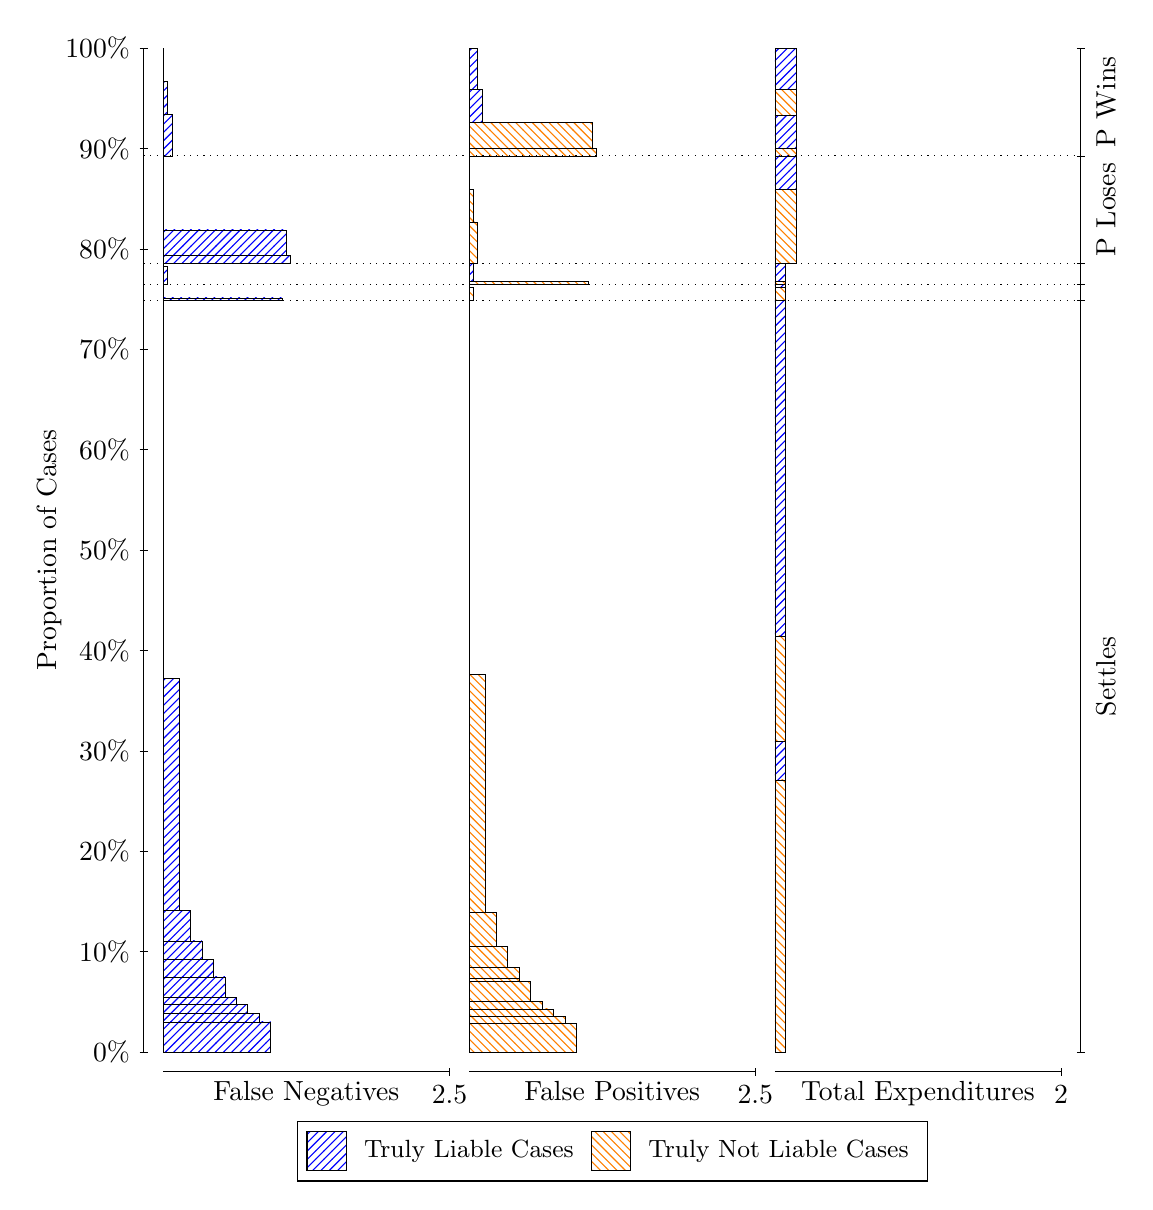
\begin{tikzpicture}
\draw[black, very thin] (1.5,1.75) -- (1.5,14.5);
\node[rotate=90, text=black, anchor=center] at (0.3, 8.125) {Proportion of Cases};
\draw[black, very thin] (1.45,1.75) -- (1.55,1.75);
\node[text=black, anchor=east] at (1.45, 1.75) {0\%};
\draw[black, very thin] (1.45,3.025) -- (1.55,3.025);
\node[text=black, anchor=east] at (1.45, 3.025) {10\%};
\draw[black, very thin] (1.45,4.3) -- (1.55,4.3);
\node[text=black, anchor=east] at (1.45, 4.3) {20\%};
\draw[black, very thin] (1.45,5.575) -- (1.55,5.575);
\node[text=black, anchor=east] at (1.45, 5.575) {30\%};
\draw[black, very thin] (1.45,6.85) -- (1.55,6.85);
\node[text=black, anchor=east] at (1.45, 6.85) {40\%};
\draw[black, very thin] (1.45,8.125) -- (1.55,8.125);
\node[text=black, anchor=east] at (1.45, 8.125) {50\%};
\draw[black, very thin] (1.45,9.4) -- (1.55,9.4);
\node[text=black, anchor=east] at (1.45, 9.4) {60\%};
\draw[black, very thin] (1.45,10.675) -- (1.55,10.675);
\node[text=black, anchor=east] at (1.45, 10.675) {70\%};
\draw[black, very thin] (1.45,11.95) -- (1.55,11.95);
\node[text=black, anchor=east] at (1.45, 11.95) {80\%};
\draw[black, very thin] (1.45,13.225) -- (1.55,13.225);
\node[text=black, anchor=east] at (1.45, 13.225) {90\%};
\draw[black, very thin] (1.45,14.5) -- (1.55,14.5);
\node[text=black, anchor=east] at (1.45, 14.5) {100\%};

\draw[black, very thin] (13.4,1.75) -- (13.4,14.5);
\draw[black, very thin] (13.35,1.75) -- (13.45,1.75);
\node[anchor=west] at (13.35, 1.75) {};
\draw[black, very thin] (13.35,11.293) -- (13.45,11.293);
\node[anchor=west] at (13.35, 11.293) {};
\draw[black, very thin] (13.35,11.497) -- (13.45,11.497);
\node[anchor=west] at (13.35, 11.497) {};
\draw[black, very thin] (13.35,11.765) -- (13.45,11.765);
\node[anchor=west] at (13.35, 11.765) {};
\draw[black, very thin] (13.35,13.131) -- (13.45,13.131);
\node[anchor=west] at (13.35, 13.131) {};
\draw[black, very thin] (13.35,14.5) -- (13.45,14.5);
\node[anchor=west] at (13.35, 14.5) {};

\draw[black, very thin, pattern color=blue, pattern=north east lines] (1.75,1.75) rectangle (3.1125,2.1308);
\draw[black, very thin, pattern color=blue, pattern=north east lines] (1.75,2.1308) rectangle (2.9672,2.2379);
\draw[black, very thin, pattern color=blue, pattern=north east lines] (1.75,2.2379) rectangle (2.8218,2.3546);
\draw[black, very thin, pattern color=blue, pattern=north east lines] (1.75,2.3546) rectangle (2.6765,2.4429);
\draw[black, very thin, pattern color=blue, pattern=north east lines] (1.75,2.4429) rectangle (2.5312,2.7038);
\draw[black, very thin, pattern color=blue, pattern=north east lines] (1.75,2.7038) rectangle (2.3858,2.9258);
\draw[black, very thin, pattern color=blue, pattern=north east lines] (1.75,2.9258) rectangle (2.2405,3.1611);
\draw[black, very thin, pattern color=blue, pattern=north east lines] (1.75,3.1611) rectangle (2.0952,3.5507);
\draw[black, very thin, pattern color=blue, pattern=north east lines] (1.75,3.5507) rectangle (1.9498,6.4975);
\draw[black, very thin, pattern color=orange, pattern=north west lines] (1.75,6.4975) rectangle (1.75,11.293);
\draw[black, very thin, pattern color=blue, pattern=north east lines] (1.75,11.293) rectangle (3.2578,11.327);
\draw[black, very thin, pattern color=orange, pattern=north west lines] (1.75,11.327) rectangle (1.75,11.497);
\draw[black, very thin, pattern color=blue, pattern=north east lines] (1.75,11.497) rectangle (1.8045,11.722);
\draw[black, very thin, pattern color=orange, pattern=north west lines] (1.75,11.722) rectangle (1.75,11.765);
\draw[black, very thin, pattern color=blue, pattern=north east lines] (1.75,11.765) rectangle (3.3668,11.864);
\draw[black, very thin, pattern color=blue, pattern=north east lines] (1.75,11.864) rectangle (3.3123,12.191);
\draw[black, very thin, pattern color=orange, pattern=north west lines] (1.75,12.191) rectangle (1.75,13.131);
\draw[black, very thin, pattern color=blue, pattern=north east lines] (1.75,13.131) rectangle (1.859,13.66);
\draw[black, very thin, pattern color=blue, pattern=north east lines] (1.75,13.66) rectangle (1.8045,14.075);
\draw[black, very thin, pattern color=orange, pattern=north west lines] (1.75,14.075) rectangle (1.75,14.5);
\draw[black, very thin, pattern color=orange, pattern=north west lines] (5.6333,1.75) rectangle (6.9958,2.1169);
\draw[black, very thin, pattern color=orange, pattern=north west lines] (5.6333,2.1169) rectangle (6.8505,2.2046);
\draw[black, very thin, pattern color=orange, pattern=north west lines] (5.6333,2.2046) rectangle (6.7052,2.2984);
\draw[black, very thin, pattern color=orange, pattern=north west lines] (5.6333,2.2984) rectangle (6.5598,2.393);
\draw[black, very thin, pattern color=orange, pattern=north west lines] (5.6333,2.393) rectangle (6.4145,2.6504);
\draw[black, very thin, pattern color=orange, pattern=north west lines] (5.6333,2.6504) rectangle (6.2692,2.6869);
\draw[black, very thin, pattern color=orange, pattern=north west lines] (5.6333,2.6869) rectangle (6.2692,2.8255);
\draw[black, very thin, pattern color=orange, pattern=north west lines] (5.6333,2.8255) rectangle (6.1238,3.0893);
\draw[black, very thin, pattern color=orange, pattern=north west lines] (5.6333,3.0893) rectangle (5.9785,3.5257);
\draw[black, very thin, pattern color=orange, pattern=north west lines] (5.6333,3.5257) rectangle (5.8332,6.5455);
\draw[black, very thin, pattern color=blue, pattern=north east lines] (5.6333,6.5455) rectangle (5.6333,11.293);
\draw[black, very thin, pattern color=orange, pattern=north west lines] (5.6333,11.293) rectangle (5.6878,11.463);
\draw[black, very thin, pattern color=blue, pattern=north east lines] (5.6333,11.463) rectangle (5.6333,11.497);
\draw[black, very thin, pattern color=orange, pattern=north west lines] (5.6333,11.497) rectangle (7.1412,11.54);
\draw[black, very thin, pattern color=blue, pattern=north east lines] (5.6333,11.54) rectangle (5.6878,11.765);
\draw[black, very thin, pattern color=orange, pattern=north west lines] (5.6333,11.765) rectangle (5.7423,12.293);
\draw[black, very thin, pattern color=orange, pattern=north west lines] (5.6333,12.293) rectangle (5.6878,12.706);
\draw[black, very thin, pattern color=blue, pattern=north east lines] (5.6333,12.706) rectangle (5.6333,13.131);
\draw[black, very thin, pattern color=orange, pattern=north west lines] (5.6333,13.131) rectangle (7.2502,13.23);
\draw[black, very thin, pattern color=orange, pattern=north west lines] (5.6333,13.23) rectangle (7.1957,13.557);
\draw[black, very thin, pattern color=blue, pattern=north east lines] (5.6333,13.557) rectangle (5.7968,13.971);
\draw[black, very thin, pattern color=blue, pattern=north east lines] (5.6333,13.971) rectangle (5.7423,14.5);
\draw[black, very thin, pattern color=orange, pattern=north west lines] (9.5167,1.75) rectangle (9.6529,5.2062);
\draw[black, very thin, pattern color=blue, pattern=north east lines] (9.5167,5.2062) rectangle (9.6529,5.694);
\draw[black, very thin, pattern color=orange, pattern=north west lines] (9.5167,5.694) rectangle (9.6529,7.0334);
\draw[black, very thin, pattern color=blue, pattern=north east lines] (9.5167,7.0334) rectangle (9.6529,11.293);
\draw[black, very thin, pattern color=orange, pattern=north west lines] (9.5167,11.293) rectangle (9.6529,11.463);
\draw[black, very thin, pattern color=blue, pattern=north east lines] (9.5167,11.463) rectangle (9.6529,11.497);
\draw[black, very thin, pattern color=orange, pattern=north west lines] (9.5167,11.497) rectangle (9.6529,11.54);
\draw[black, very thin, pattern color=blue, pattern=north east lines] (9.5167,11.54) rectangle (9.6529,11.765);
\draw[black, very thin, pattern color=orange, pattern=north west lines] (9.5167,11.765) rectangle (9.7892,12.706);
\draw[black, very thin, pattern color=blue, pattern=north east lines] (9.5167,12.706) rectangle (9.7892,13.131);
\draw[black, very thin, pattern color=orange, pattern=north west lines] (9.5167,13.131) rectangle (9.7892,13.23);
\draw[black, very thin, pattern color=blue, pattern=north east lines] (9.5167,13.23) rectangle (9.7892,13.645);
\draw[black, very thin, pattern color=orange, pattern=north west lines] (9.5167,13.645) rectangle (9.7892,13.971);
\draw[black, very thin, pattern color=blue, pattern=north east lines] (9.5167,13.971) rectangle (9.7892,14.5);
\draw[black, dotted] (1.5,11.293) -- (13.4,11.293);
\draw[black, dotted] (1.5,11.497) -- (13.4,11.497);
\draw[black, dotted] (1.5,11.765) -- (13.4,11.765);
\draw[black, dotted] (1.5,13.131) -- (13.4,13.131);
\draw[black, very thin] (1.75,1.5) -- (5.3833,1.5);
\node[text=black, anchor=north] at (3.5667, 1.5) {False Negatives};
\draw[black, very thin] (5.3833,1.45) -- (5.3833,1.55);
\node[text=black, anchor=north] at (5.3833, 1.45) {2.5};

\draw[black, very thin] (5.6333,1.5) -- (9.2667,1.5);
\node[text=black, anchor=north] at (7.45, 1.5) {False Positives};
\draw[black, very thin] (9.2667,1.45) -- (9.2667,1.55);
\node[text=black, anchor=north] at (9.2667, 1.45) {2.5};

\draw[black, very thin] (9.5167,1.5) -- (13.15,1.5);
\node[text=black, anchor=north] at (11.333, 1.5) {Total Expenditures};
\draw[black, very thin] (13.15,1.45) -- (13.15,1.55);
\node[text=black, anchor=north] at (13.15, 1.45) {2};

\node[text=black, centered, rotate=90] at (13.72, 6.5215) {Settles};


\node[text=black, centered, rotate=90] at (13.72, 12.448) {P Loses};
\node[text=black, centered, rotate=90] at (13.72, 13.816) {P Wins};

\draw (7.449999999999999,1.5) node[draw=none] (baseCoordinate) {};
\begin{scope}[align=center]
        \matrix[scale=0.5, draw=black, below=0.5cm of baseCoordinate, nodes={draw}, column sep=0.1cm]{
            \node[rectangle, draw, minimum width=0.5cm, minimum height=0.5cm, pattern color=blue, pattern=north east lines] {}; &
            \node[draw=none, font=\small, text=black] (B) {Truly Liable Cases}; &
            \node[rectangle, draw, minimum width=0.5cm, minimum height=0.5cm, pattern color=orange, pattern=north west lines] {}; &
            \node[draw=none, font=\small, text=black] (B) {Truly Not Liable Cases}; \\
            };
\end{scope}

\end{tikzpicture}
\end{document}